\documentclass[main.tex]{subfiles}

\begin{document}
The purpose of the researchers in the past year was to find a easy way to generate all the possible rhythms present in music, in order to extend the dictionary of Automatic Music Composition\cite{Allouche:2002:AutomSeq:book}.
Before proceeding with the implementation of the drum machine, it’s necessary to dwelve into the algorithm of Euclid and explain what it has to do with rhythm generation.\\
In order to compute the greatest common divisor between two integers, the greek mathematician proposed this solution: the smaller number is repeatedly subtracted from the greater until the greater is zero or becomes smaller than the smaller, in which case it is called the remainder. This remainder is then repeatedly subtracted from the smaller number to obtain a new remainder. This process is continued until the remainder is zero\cite{Euclid:Elements}. 
The same procedure can be done more efficiently with divisions.\\
[2mm]
\begin{algorithm}
\label{euclid}
\begin{algorithmic}[1]
\Procedure{euclid}{$m,k$}
\If {$k == 0$}
\State \Return $m$
\Else
\State \Return{\Call {euclid}{$k, m \mod k$}}

\EndIf
\EndProcedure
\end{algorithmic}
\end{algorithm}\\
[3mm]
The derivation of G. Touissant\cite{Toussaint:2004:euclidean:rhythm} comes from an analyisis over Bjorklund's studies on SNS accelerators\cite{Bjorklund:2003:euclidean:rhythm} in nuclear physics. In this case, time is divided into intervals and during some of these intervals an onset is to be enabled by a timing system that generates pulses that accomplish this task. The problem for a given number \textit{n} of time intervals, and another given number \begin{math}k<n\end{math} of pulses, is to distribute the pulses as evenly as possible among these intervals.\\
In our case the algorithm to be develped take as input a tuple \begin{math}{(k, n)}\end{math}, where \begin{math}{n}\end{math} represents the length of the played sequence and \begin{math}{k}\end{math} the number of onsets inside the sequence. The output is a sequence of length \begin{math}{n}\end{math}, where the \begin{math}{k}\end{math} onsets are equally spaced inside the sequence. For example, if we consider the tuple \begin{math}{(4, 16)}\end{math}, the result has to be a sequence like:\\
[2mm]
[1, 0, 0, 0, 1, 0, 0, 0, 1, 0, 0, 0, 1, 0, 0, 0]\\
[3mm]
As Touissant explains in his work\cite{Toussaint:2004:euclidean:rhythm}, with this mechanism we can produce all the possible rhythmic sequences, linking them to a specific musical genre(\autoref{fig:1}). For instance:
\begin{itemize}[noitemsep]
\item \begin{math}E(2,3)=[1,0,1]\end{math} is a common Afro-Cuban drum pattern. For example, it is the conga rhythm of the (6/8)-time Swing Tumbao\cite{Klower:1997}.
\item \begin{math}E(2,5)=[1,0,1,0,0]\end{math}, when it is started on the second onset (\begin{math}[1,0,0,1,0]\end{math}) is the metric pattern of Dave Brubeck’s \textit{Take Five} as well as \textit{Mars} from \textit{The Planets} by Gustav Holst\cite{Keith:1991}.
\item \begin{math}E(5,16)=[1,0,0,1,0,0,1,0,0,1,0,0,1,0,0,0]\end{math} is the Bossa-Nova rhythm necklace of Brazil, started on the second onset\cite{Behague:1973}.
\end{itemize}

\begin{figure}[htbp]
\centering
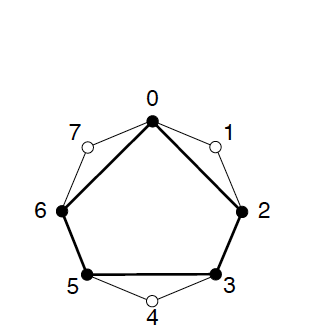
\includegraphics{images/cuban_cinquillo.png}
\caption{The Euclidean rhythm $E(5,8)$ of the Cuban cinquillo}
\label{fig:1}
\end{figure}
The application uses as reference the algorithm explained by Bjorklund\cite{Bjorklund:2003:euclidean:rhythm}. It is composed by two steps: the first consists in creating the base string and the second in spacing the onsets inside the base string.\\
Considering \begin{math}m\end{math} the length of sequence and \begin{math}n\end{math} the number of onsets, and supposing that \begin{math}n<\frac{m}{2}\end{math}, we need to create a sequence of \begin{math}m-n\end{math} zeros and one another of \begin{math}n\end{math} ones. In the case of five pulses of thirteen cycles, we start from seqeuences \begin{math}[00000000]\end{math} and \begin{math}[11111]\end{math}.\\
We start by simply dividing the five 1’s into the eight 0’s. This will put a 1 after every 0, with three 0’s left over: \begin{math}[0101010101]\end{math} and \begin{math}[000]\end{math}.\\
Once again, we can think of this as two optimally distributed strings. One strings is ten bits long and contains five “01” pairs (an optimal distribution of five pulses over ten slots). The second string contains three 0’s. If we now distribute the three 0’s over the five “01” pairs, we get three “010” triples with two “01” pairs left over: \begin{math}[010][010][010] [01][01]\end{math}.\\
We still have two optimally distributed strings. “010010010” is an optimal distribution of three pulses over nine slots and “0101” is an optimal distribution of two pulses over four slots. We now repeat the process, dividing the two “01” strings into the three “010” strings. This gives us two five-bit strings (“01001”) with one three-bit string (“010”) as a remainder: \begin{math}[01001][01001] [010][01]\end{math}.\\
We can stop the process when the remainder reaches one or zero. Our final pattern, therefore, is \begin{math}[0100101001010]\end{math} , which is as evenly as we can distribute five pulses over thirteen slots.
\end{document}

%Before proceeding with the implementation of the drum machine, it’s necessary to dwelve into the algorithm of Euclid and explain what it has to do with rhythm generation.
 %In order to compute the greatest common divisor between two integers, the greek mathematician proposed this solution:
%The smaller number is repeatedly subtracted from the greater until the greater is zero or becomes smaller than the smaller, in which case it is called the remainder. This remainder is then repeatedly subtracted from the smaller number to obtain a new remainder. This process is continued until the remainder is zero. 
%The same procedure can be done more efficiently with divisions.

%EUCLID(m, k)
 %1. if k = 0
 %2. then return m 
 %3. else return EUCLID(k,m mod k)
%If m and k are intended as the number of zero’s and one’s, respectively, in a binary sequence (with n = m+k), the structure of this algorithm can be exploited to produce an array of zero’s and one’s and use the one’s as the onset in a rhythmic pattern. In this case m will be the greater number,  and it will represent the sequence length, k will represent the number of onsets to distribute as evenly as possible in the sequence.
%As an example ….
%It is also well known that if algorithm EUCLID(m, k) is applied to two O(n) bit numbers (binary sequences of length n) it will perform O(n) arithmetic operations in the worst case [8 del paper euclideo]